\subsection{Lab22: Python block}

%*********************
\begin{frame}{}

\pgfdeclareimage[width=\paperwidth,height=\paperheight]{bg}{imagenes/fondo_lab}
\setbeamertemplate{background}{\pgfuseimage{bg}}

\bfseries{\textrm{\LARGE Actividad\\ \Large Embedded Python Block}}
\raggedright
\end{frame}
%*********************

%--------------------------

\begin{frame}{Python block }


\pgfdeclareimage[width=\paperwidth,height=\paperheight]{bg}{imagenes/fondo3}
\setbeamertemplate{background}{\pgfuseimage{bg}}

  \begin{itemize}
  \item \justifying Le permite crear un nuevo bloque (personalizado) en Python sin necesidad de crear e instalar un Módulo fuera del árbol (OOT). Cuando agrega el bloque a su diagrama de flujo, el código rellenado previamente simplemente toma el flujo de entrada y lo multiplica por una constante. Tenga en cuenta que la estructura de este bloque de Python coincide con la estructura de un bloque de Python fuera del árbol (OOT) Es esencialmente un bloque Python OOT integrado en un diagrama de flujo grc.


 
  \end{itemize}
\end{frame}
%---------------------------

\begin{frame}{Python block}

\begin{figure}[H]
\centering
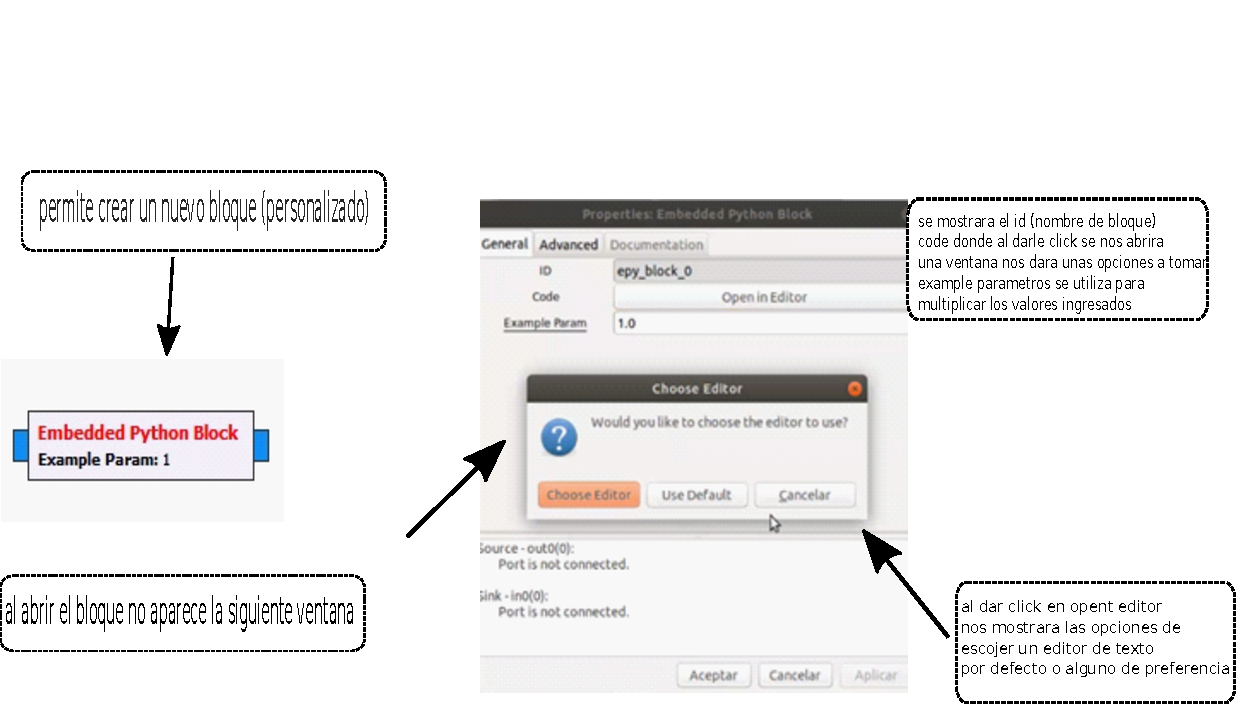
\includegraphics[width=\textwidth]{Modulaciones_digitales/lab22/pdf/lab22.pdf}
\end{figure}
\end{frame}
%--------------------


\begin{frame}{Python block }


\pgfdeclareimage[width=\paperwidth,height=\paperheight]{bg}{imagenes/fondo3}
\setbeamertemplate{background}{\pgfuseimage{bg}}

  \begin{itemize}
  \item \justifying Después de haber elegido nuestro editor por defecto o editor de texto preferente se nos genera un codigo del bloque. en el cual se ingresaran los parametros como se observara a continuacion en el ejemplo


 
  \end{itemize}
\end{frame}
%---------------------------

\begin{frame}{Python block}
\vspace{-1cm}
\begin{figure}[H]
\centering
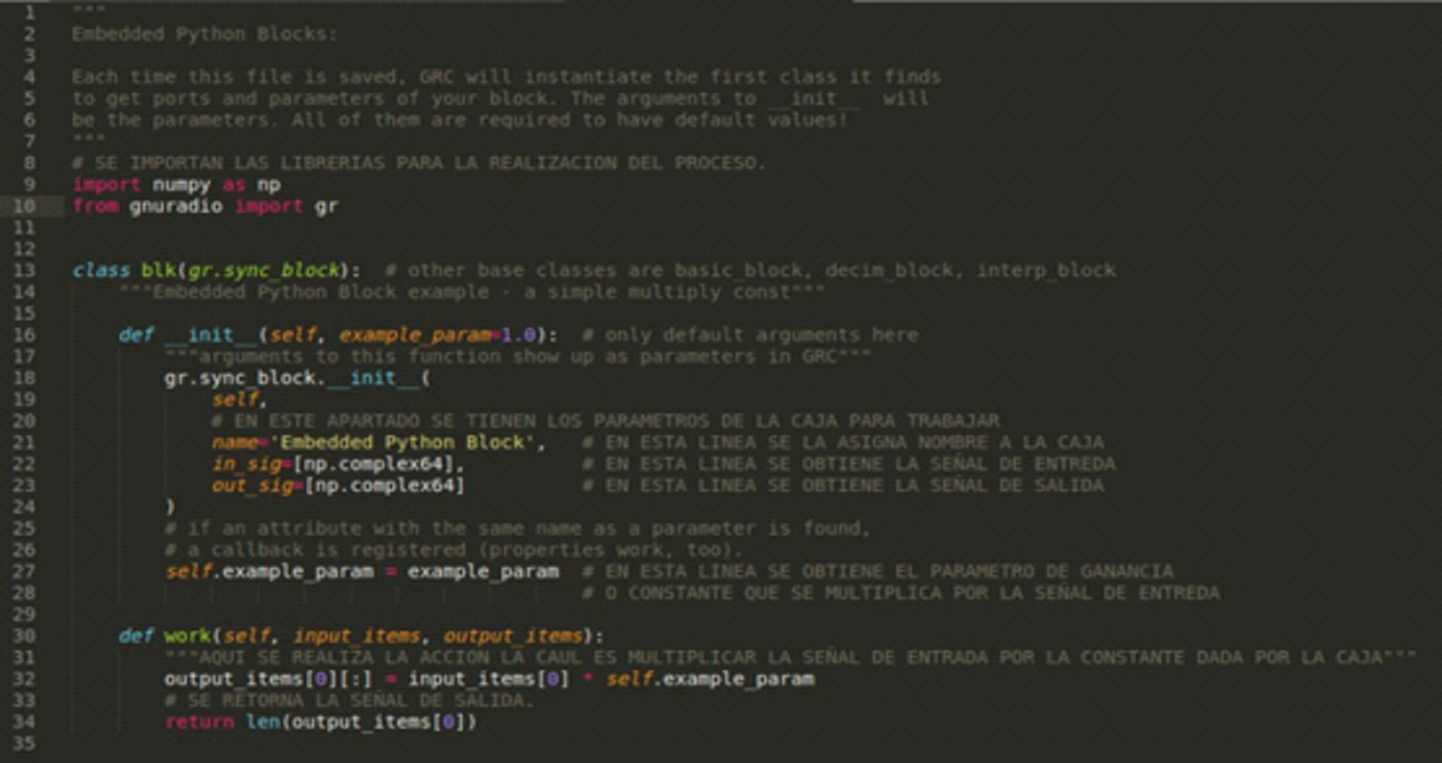
\includegraphics[width=1.1\textwidth]{Modulaciones_digitales/lab22/pdf/lab22_1.pdf}
\end{figure}
\end{frame}
%_---------------------

\begin{frame}{Python block}
\vspace{-1.5cm}
\begin{figure}[H]
\centering
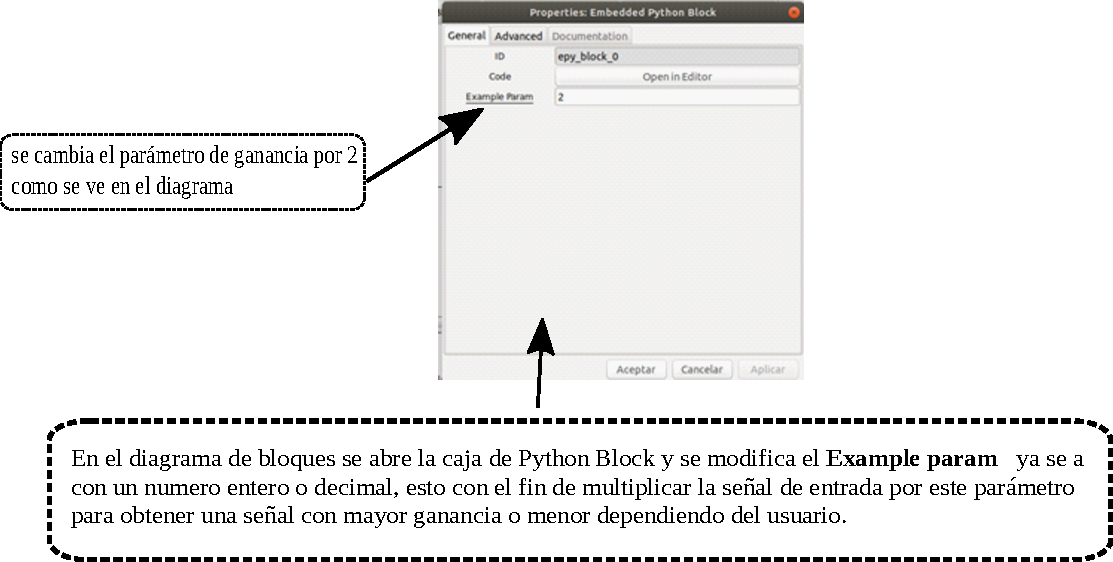
\includegraphics[width=1.1\textwidth]{Modulaciones_digitales/lab22/pdf/lab22_2.pdf}
\end{figure}
\end{frame}
%_---------------------
%_---------------------

\begin{frame}{Python block}
\vspace{-1.5cm}
\begin{figure}[H]
\centering
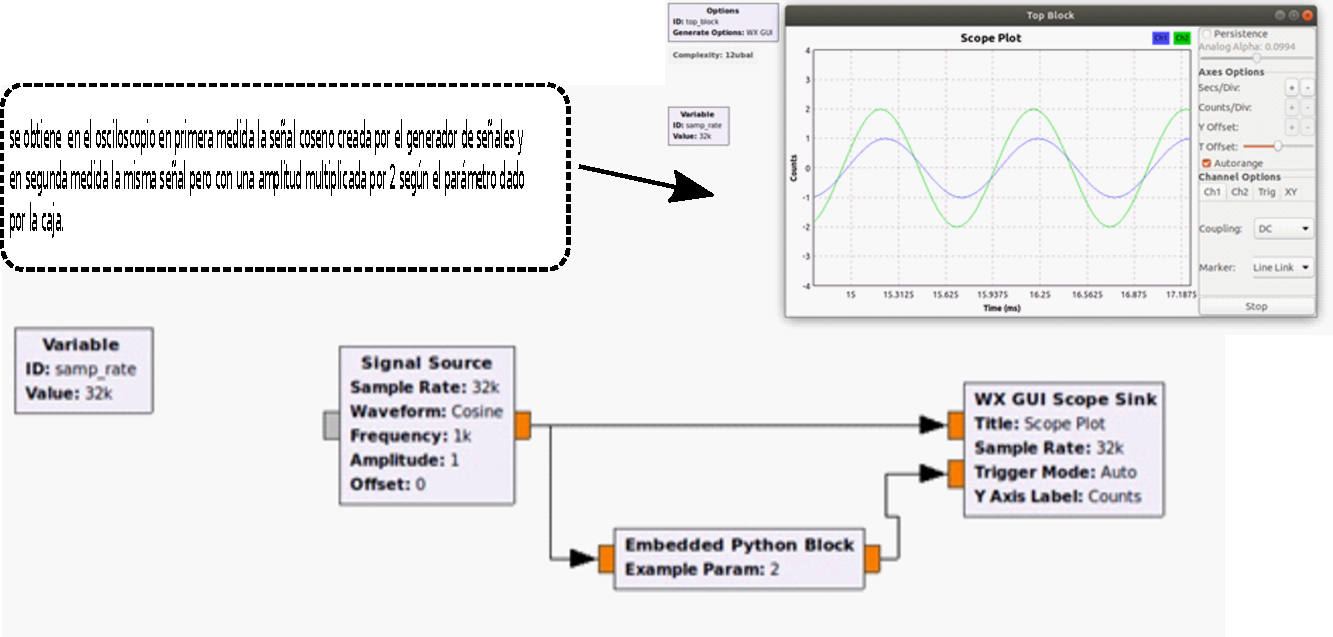
\includegraphics[width=1.1\textwidth]{Modulaciones_digitales/lab22/pdf/lab22_3.pdf}
\end{figure}
\end{frame}
%_---------------------
